\section{System Base Description}
\label{sec:Vehicledescription}
The technology which has been provided for the prototype is a tracked vehicle, seen on \figref{TrackedVehicle}, a battery and a GoT system. A platform with the length and width of the vehicle is mounted on the vehicle to protect the mechanical system. This is utilized to support the rest of the system, which includes PCB boards, the battery, and the sensors used to control the vehicle. When the platform is mounted on, the vehicle is 45 cm long, 29 cm in width, 12 cm in height and weighs 2932 grams.
%
\begin{figure}[H]
	\centering
	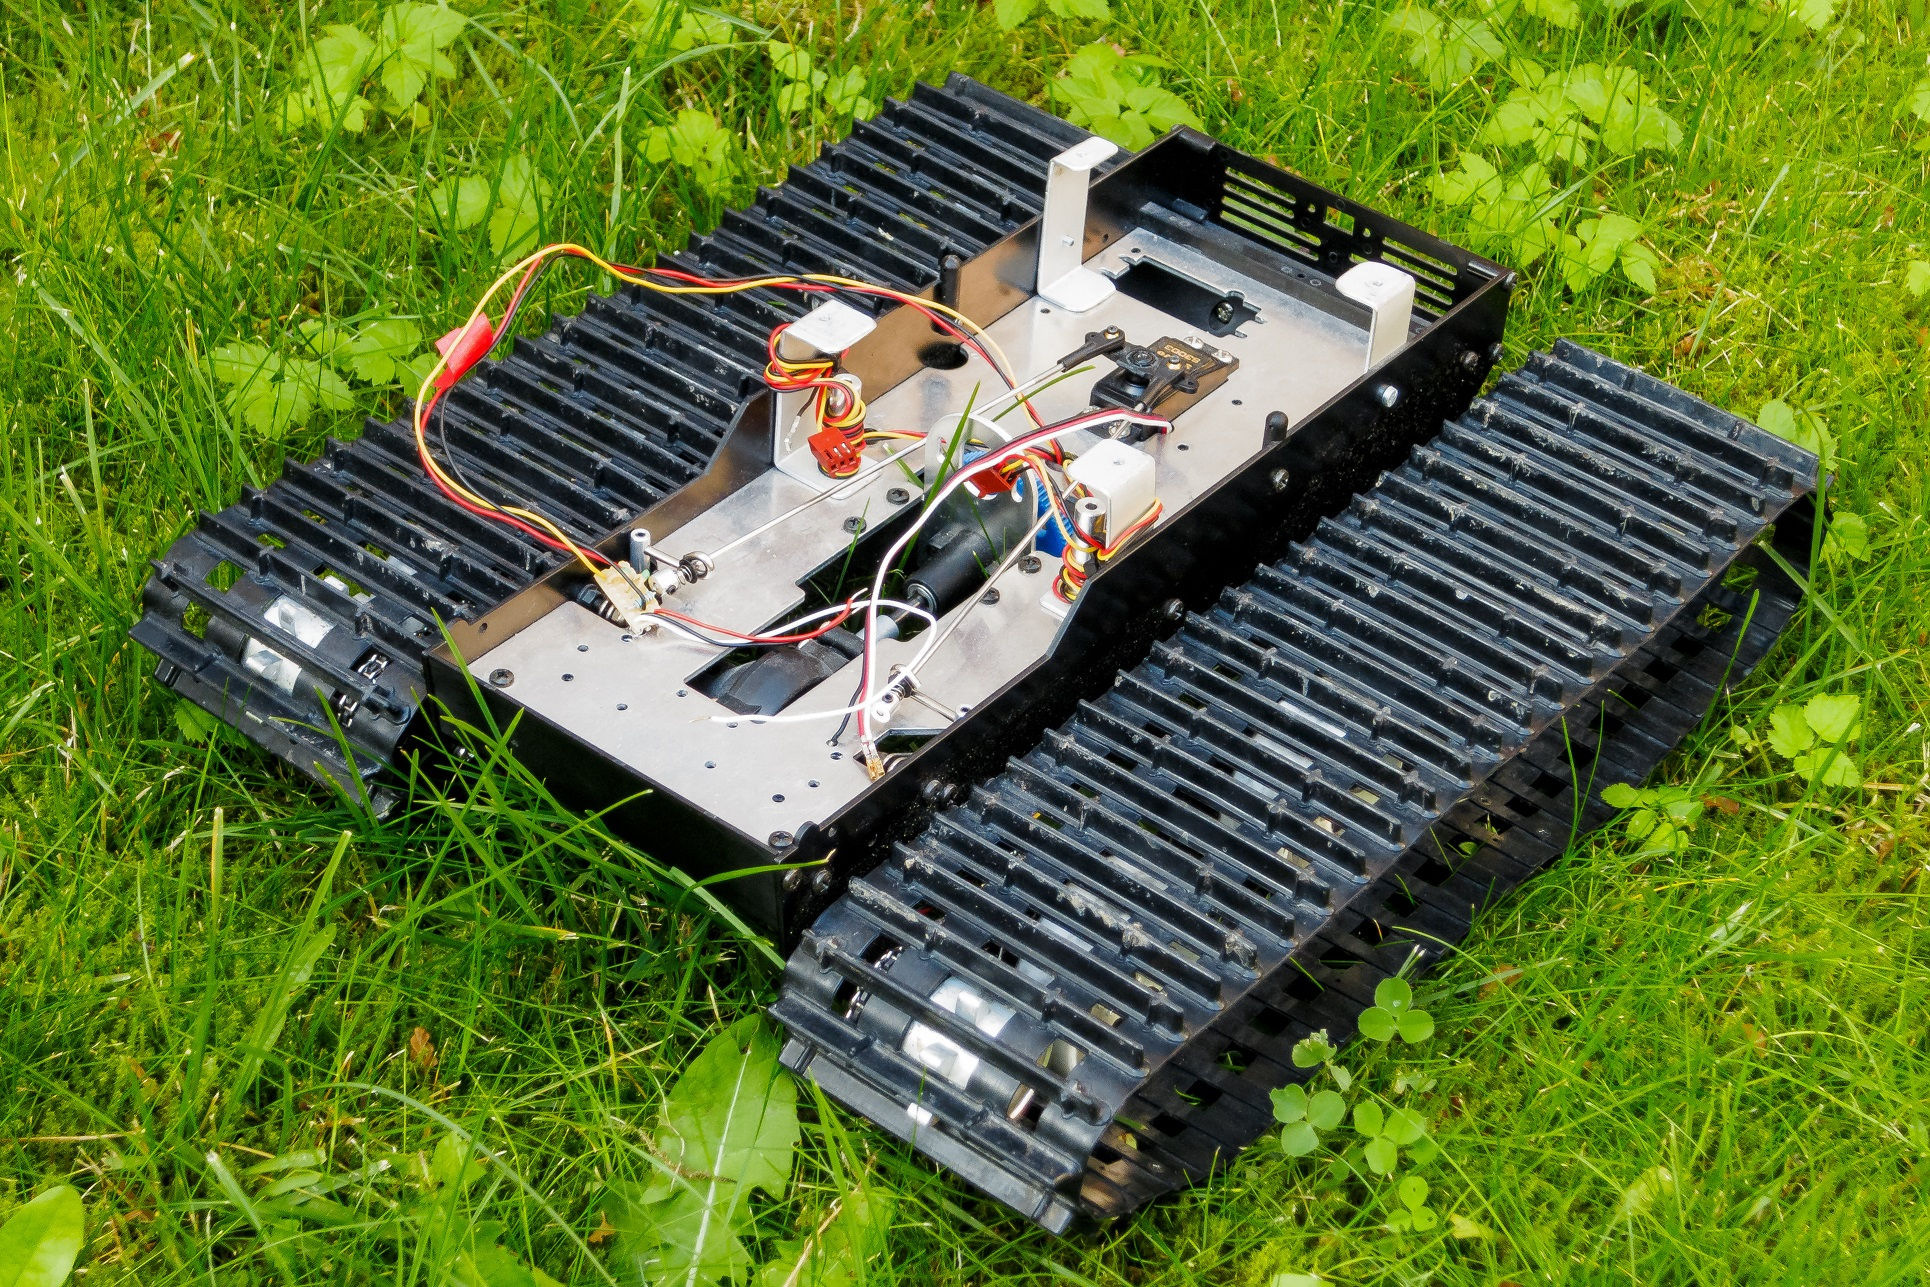
\includegraphics[scale=0.6]{figures/BeltVehicle.jpg}
	\caption{The provided tracked vehicle without a platform}
	\label{TrackedVehicle}
\end{figure}\vspace{-5mm}
%
To get an understanding of how the motor is used to make the belts rotate, one must comprehend how the drivetrain, see \figref{FullVehicle}, functions. To make the vehicle turn it is necessary to understand how the servo acts on the brakes, which are connected to the driving wheels on each side of the vehicle. Two Hall sensors are attached to the provided vehicle, along with 4 magnets attached to each drive gear. To run the vehicle a rechargeable battery pack is also provided. Furthermore it is necessary to understand how the GoT system works to be able to utilize it and thereby be able to track the vehicle.

First a description of the vehicle's drivetrain will be given.